\documentclass{article}

\usepackage{graphicx}
\usepackage{tikz}
\usepackage{tikzsymbols}
\usetikzlibrary{calc,patterns,shapes.geometric}
\pagestyle{empty}
\usepackage[margin=0pt]{geometry}
\geometry{papersize={14in,12in}}

\def\centerarc[#1](#2)(#3:#4:#5){\draw[#1] ($(#2)+({#5*cos(#3)},{#5*sin(#3)})$) arc (#3:#4:#5);}

\begin{document}
	\begin{figure}
		\centering
		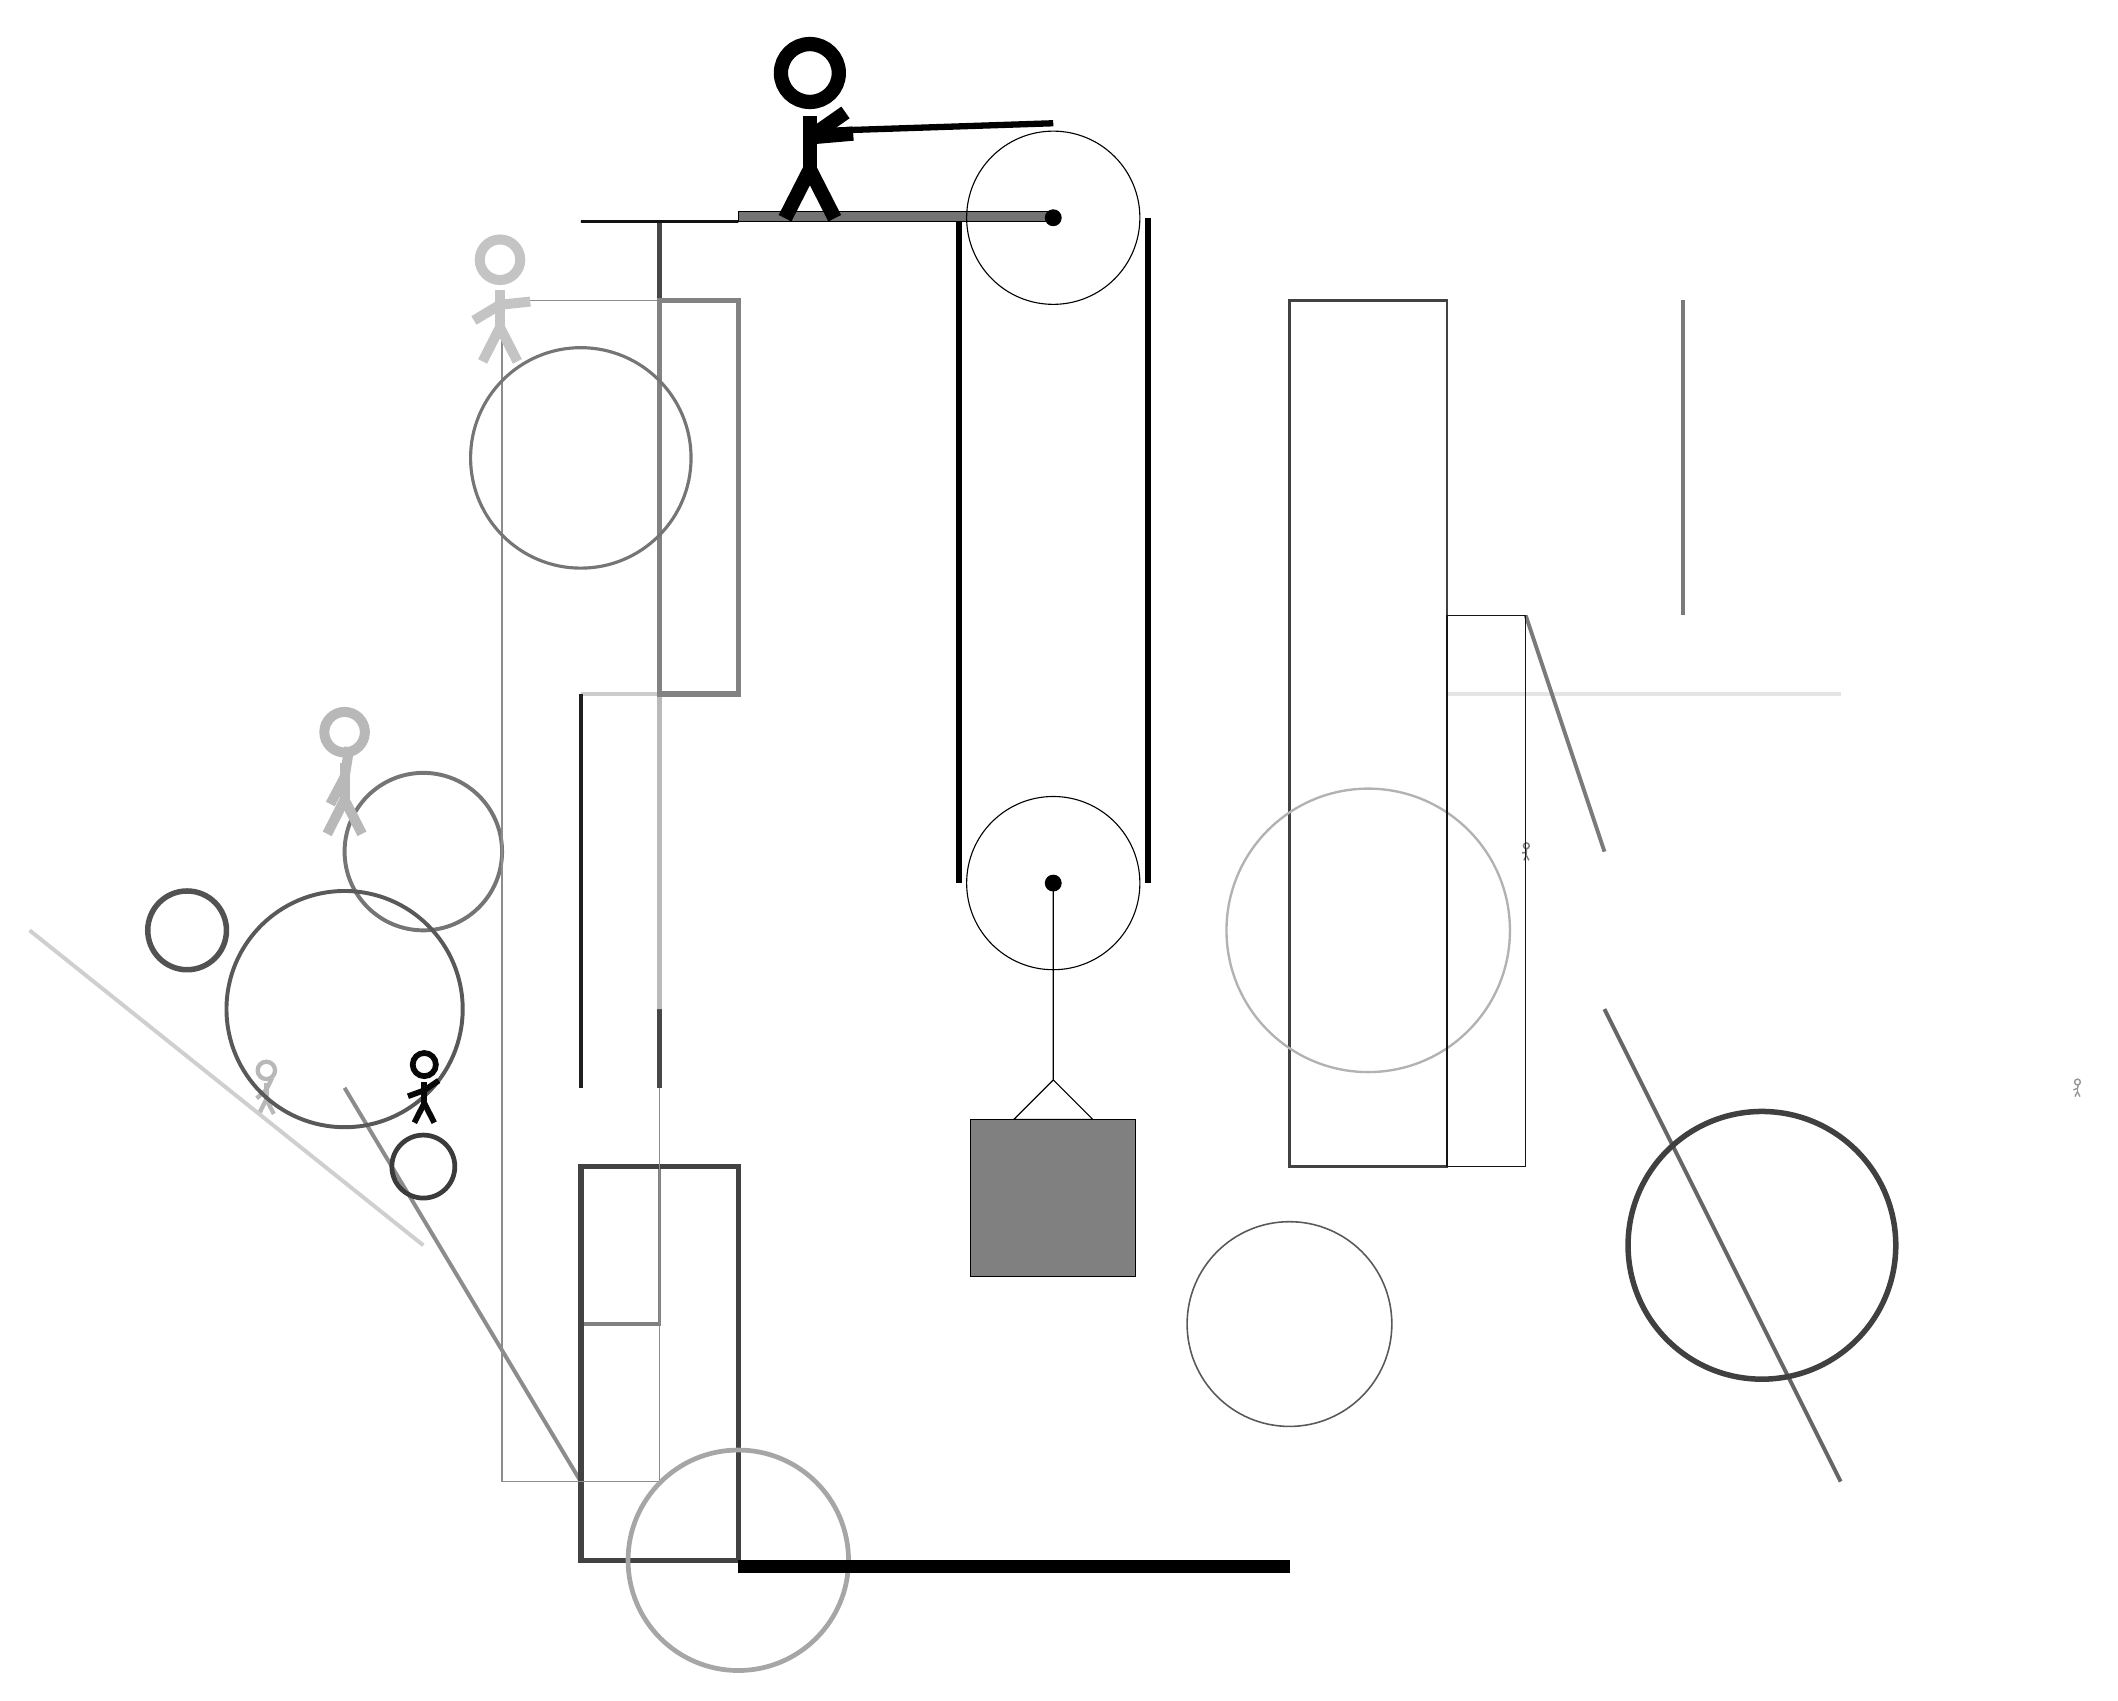
\begin{tikzpicture}
			%%%%% START %%%%%
			
			\draw[fill=black!55] (-2, 14) rectangle (2, 14.125);
			
			\draw (2, 5.6) circle (1.1);
			\draw[fill=black] (2, 5.6) circle (0.1);
			
			\draw[line width=0.5mm, color=black!45](-4, -2) -- (-7, 3);
			
			\draw[line width=0.5mm, color=black!60](9, 4) -- (12, -2);
			\draw[line width=0.4mm, color=black!50] (-3, 0) rectangle (-4, 2);
			\draw[line width=0.7mm, color=black!74] (-4, -3) rectangle (-2, 2);
			\draw [line width=0.5mm, color=black!54](-6, 6) circle (1.0);
			\draw [line width=0.6mm, color=black!77](-6, 2) circle (0.4);
			\draw[line width=0.5mm, color=black!20] (-4, 8) rectangle (-2, 8);
			\draw[line width=0.2mm, color=black!45] (-3, 13) rectangle (-5, -2);
			\node[line width=0.7mm, color=black!28] at (-8, 3) {\Strichmaxerl[3][42][64]};
			\draw [line width=0.7mm, color=black!75](11, 1) circle (1.7);
			
			\node[line width=0.6mm, color=black!53] at (8, 6) {\Strichmaxerl[1][10][87]};
			\draw[line width=0.3mm, color=black!74] (5, 2) rectangle (7, 13);
			\draw [line width=0.2mm, color=black!65](5, 0) circle (1.3);
			
			\draw[line width=0.5mm, color=black!52](10, 13) -- (10, 9);
			\draw [line width=0.6mm, color=black!35](-2, -3) circle (1.4);
			\draw [line width=0.5mm, color=black!65](-7, 4) circle (1.5);
			
			\draw[line width=0.7mm, color=black!72] (-3, 14) rectangle (-3, 3);
			\node[line width=0.4mm, color=black!97] at (-6, 3) {\Strichmaxerl[4][20][34]};
			\node[line width=0.7mm, color=black!41] at (15, 3) {\Strichmaxerl[1][19][77]};
			
			\draw[line width=0.5mm, color=black!19](-6, 1) -- (-11, 5);
			\draw[line width=0.7mm, color=black!27] (-3, 4) rectangle (-3, 9);
			
			\draw[line width=0.7mm, color=black!49] (-3, 8) rectangle (-2, 13);
			\node[line width=0.5mm, color=black!23] at (-5, 13) {\Strichmaxerl[7][31][6]};
			\draw [line width=0.4mm, color=black!54](-4, 11) circle (1.4);
			\draw[line width=0.5mm, color=black!10](7, 8) -- (12, 8);
			
			\draw[line width=0.5mm, color=black!88] (-4, 8) rectangle (-4, 3);
			
			\draw [line width=0.7mm, color=black!68](-9, 5) circle (0.5);
			\node[line width=0.5mm, color=black!28] at (-7, 7) {\Strichmaxerl[7][62][81]};
			
			\draw [line width=0.3mm, color=black!30](6, 5) circle (1.8);
			\draw[line width=0.4mm, color=black!93] (-2, 14) rectangle (-4, 14);
			\draw[line width=0.5mm, color=black!52](9, 6) -- (8, 9);
			
			\draw[line width=0.2mm, color=black!92] (7, 2) rectangle (8, 9);
			
			\draw (2, 14.05) circle (1.1);
			\draw[fill=black] (2, 14.05) circle (0.1);
			
			\draw (2, 5.6) -- (2, 3.1) -- (1.5, 2.6) -- (2.5, 2.6) -- (2, 3.1);
			\draw[fill=black!50] (0.95, 2.6) rectangle (3.05, 0.6);
			
			\draw[line width=0.8mm] (0.8, 14) -- (0.8, 5.6);
			\centerarc[line width=0.8mm](2, 5.6)(180:360:1.2000000000000002);
			\draw[line width=0.8mm](3.2, 5.6) -- (3.2, 14.05);
			\centerarc[line width=0.8mm](2, 14.05)(0:90:1.2000000000000002);
			\draw[line width=0.8mm](2, 15.25) -- (-1, 15.15);
			
			\node at (-1, 15.15) {\Strichmaxerl[10][-175][35]};
			
			\draw[fill=black] (-2, -3) rectangle (5, -3.15);
			
			%%%%% END %%%%%
		\end{tikzpicture}
	\end{figure}	
\end{document}